\documentclass[aspectratio=169,10pt]{beamer}
\usetheme{Madrid}
\usecolortheme{default}

% Packages
\usepackage[english]{babel}
\usepackage{amsmath}
\usepackage{amssymb}
\usepackage{graphicx}
\usepackage{siunitx}
\usepackage{physics}
\usepackage{listings}
\usepackage{xcolor}
\usepackage{tikz}
\usepackage{hyperref}

% Custom colors
\definecolor{acousticblue}{RGB}{33, 150, 243}
\definecolor{acousticorange}{RGB}{255, 152, 0}
\definecolor{acousticgreen}{RGB}{76, 175, 80}

% Title information
\title[Traverso Analysis Software]{Comprehensive Acoustic Analysis Software\\for Transverse Flutes}
\subtitle{Advanced Tools for Geometric Modeling, Impedance Analysis, and Acoustic Characterization}
\author[Your Name]{Your Name}
\institute[Your Institution]{Your Institution}
\date{\today}

% Beamer settings
\setbeamertemplate{navigation symbols}{}
\setbeamertemplate{footline}[frame number]

\begin{document}

% Title slide
\begin{frame}
\titlepage
\end{frame}

% Outline
\begin{frame}{Outline}
\tableofcontents
\end{frame}

% ==================== SECTION 1: INTRODUCTION ====================
\section{Introduction}

\begin{frame}{Overview}
\begin{itemize}
    \item \textbf{Comprehensive software suite} for acoustic analysis of transverse flutes
    \item \textbf{Integration} with OpenWind library for impedance computation
    \item \textbf{Multi-flute comparison} and statistical analysis capabilities
    \item \textbf{Geometric modeling} with support for cylindrical and conical holes
    \item \textbf{Advanced acoustic metrics} for instrument characterization
\end{itemize}

\vspace{0.5cm}
\begin{block}{Key Capabilities}
    \begin{itemize}
        \item Geometric visualization (2D profiles, 3D models, engineering drawings)
        \item Acoustic impedance/admittance analysis
        \item Resonator truncation analysis (novel method)
        \item Sensitivity analysis for geometric parameters
        \item Database management and statistical reporting
    \end{itemize}
\end{block}
\end{frame}

\begin{frame}{Software Architecture}
\begin{columns}
\begin{column}{0.5\textwidth}
\textbf{Core Components:}
\begin{itemize}
    \item \texttt{FluteData} / \texttt{FluteDataDB}
    \begin{itemize}
        \item Data loading and validation
        \item Geometry concatenation
        \item Database caching
    \end{itemize}
    \item \texttt{FluteAnalyzer}
    \begin{itemize}
        \item Acoustic metrics calculation
        \item Multi-flute comparison
    \end{itemize}
    \item \texttt{ResonatorTruncationAnalyzer}
    \begin{itemize}
        \item Novel truncation analysis
    \end{itemize}
\end{itemize}
\end{column}
\begin{column}{0.5\textwidth}
\textbf{Visualization \& Tools:}
\begin{itemize}
    \item \texttt{FluteOperations}
    \begin{itemize}
        \item 2D/3D plotting
        \item Engineering drawings
    \end{itemize}
    \item \texttt{FluteGeometryEditor}
    \begin{itemize}
        \item Interactive geometry editing
    \end{itemize}
    \item \texttt{SensitivityAnalysis}
    \begin{itemize}
        \item Parameter variation studies
    \end{itemize}
\end{itemize}
\end{column}
\end{columns}

\vspace{0.3cm}
\begin{center}
\textit{Unified PyQt5 GUI integrates all components}
\end{center}
\end{frame}

% ==================== SECTION 2: GEOMETRIC VISUALIZATION ====================
\section{Geometric Visualization}

\begin{frame}{2D Geometric Profiles}
\textbf{Multiple visualization modes:}

\begin{enumerate}
    \item \textbf{Combined Profile}
    \begin{itemize}
        \item Internal acoustic profile (cork-referenced)
        \item External physical profile (with wall thickness)
        \item Hole positions and dimensions
    \end{itemize}
    
    \item \textbf{Individual Parts}
    \begin{itemize}
        \item Headjoint, left, right, foot sections
        \item Internal and external profiles per part
    \end{itemize}
    
    \item \textbf{Axial Cross-Section}
    \begin{itemize}
        \item 2D view with hole polygons
        \item Support for cylindrical and conical holes
    \end{itemize}
    
    \item \textbf{Top View}
    \begin{itemize}
        \item Concentric circles for conical holes
        \item Hole positions along the bore
    \end{itemize}
\end{enumerate}
\end{frame}

\begin{frame}{Hole Geometry Support}
\textbf{Cylindrical Holes:}
\begin{equation*}
D_{\text{hole}} = \text{constant}
\end{equation*}

\textbf{Conical Holes (Undercut):}
\begin{equation*}
D_{\text{outer}} < D_{\text{inner}}
\end{equation*}

The system automatically:
\begin{itemize}
    \item Calculates wall thickness at hole position
    \item Generates conical geometry for OpenWind
    \item Visualizes undercut angle: $\theta = \arctan\left(\frac{D_{\text{inner}} - D_{\text{outer}}}{2h}\right)$
\end{itemize}

\vspace{0.3cm}
\begin{block}{Example JSON Format}
\texttt{"Holes diameter": [12.0, [14.0, 18.0], 9.0]}\\
\textit{Cylindrical | Conical (outer, inner) | Cylindrical}
\end{block}
\end{frame}

\begin{frame}{3D Visualization}
\textbf{Interactive 3D Models:}
\begin{itemize}
    \item PyVista-based 3D rendering
    \item Internal and external geometry
    \item Multi-flute comparison in 3D space
    \item Rotatable, zoomable, interactive views
\end{itemize}

\textbf{Features:}
\begin{itemize}
    \item Lazy loading (initializes only when accessed)
    \item Part-by-part visualization
    \item Color-coded sections
    \item Export capabilities
\end{itemize}

\vspace{0.3cm}
\begin{figure}
\centering
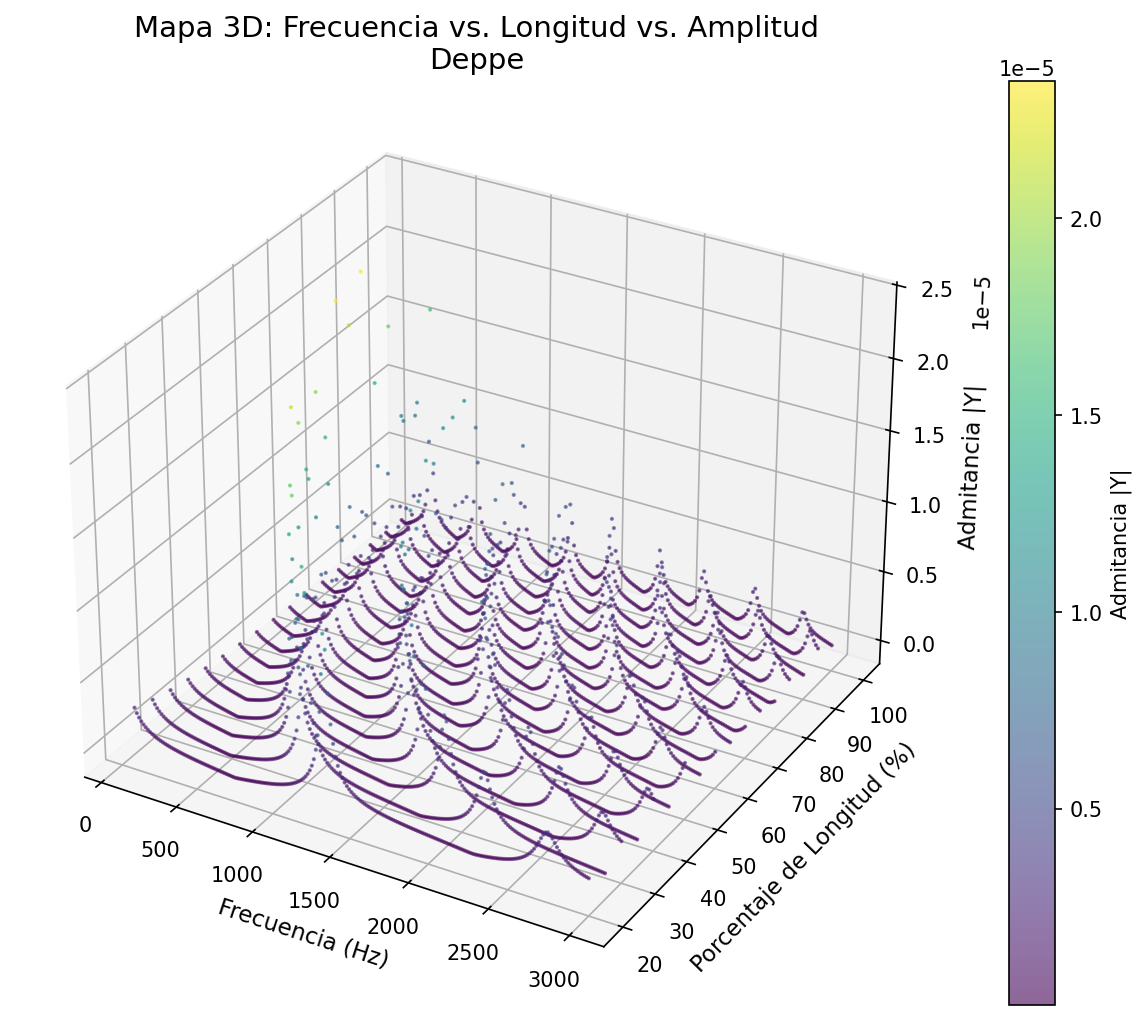
\includegraphics[width=0.65\textwidth]{presentation_screenshots/resonator_truncation_3d.png}
\end{figure}
\end{frame}

% ==================== SECTION 3: ACOUSTIC ANALYSIS ====================
\section{Acoustic Analysis}

\begin{frame}{Impedance and Admittance}
\textbf{Fundamental Quantities:}

Acoustic impedance:
\begin{equation*}
Z(\omega) = \frac{P(\omega)}{U(\omega)} = R(\omega) + jX(\omega)
\end{equation*}

Acoustic admittance:
\begin{equation*}
Y(\omega) = \frac{1}{Z(\omega)} = G(\omega) + jB(\omega)
\end{equation*}

where:
\begin{itemize}
    \item $P(\omega)$: Acoustic pressure
    \item $U(\omega)$: Volume velocity
    \item $R, X$: Resistance and reactance
    \item $G, B$: Conductance and susceptance
\end{itemize}

\textbf{Computation:} OpenWind's \texttt{ImpedanceComputation} using transmission line theory
\end{frame}

\begin{frame}{Resonance Frequencies}
\textbf{Antiresonance Frequencies:}
\begin{equation*}
f_n = \arg\min_f |Z(f)| = \arg\max_f |Y(f)|
\end{equation*}

For an ideal open-open tube:
\begin{equation*}
f_n = \frac{nc}{2L_{\text{eff},n}}
\end{equation*}

where:
\begin{itemize}
    \item $n$: Mode number (1, 2, 3, \ldots)
    \item $c$: Speed of sound ($\approx 343$ m/s at 20°C)
    \item $L_{\text{eff},n} = L + \Delta L_{\text{head},n} + \Delta L_{\text{foot},n}$: Effective length
\end{itemize}

\textbf{Visualization:} Resonance frequencies vs. musical notes, compared to equal temperament

\begin{figure}
\centering
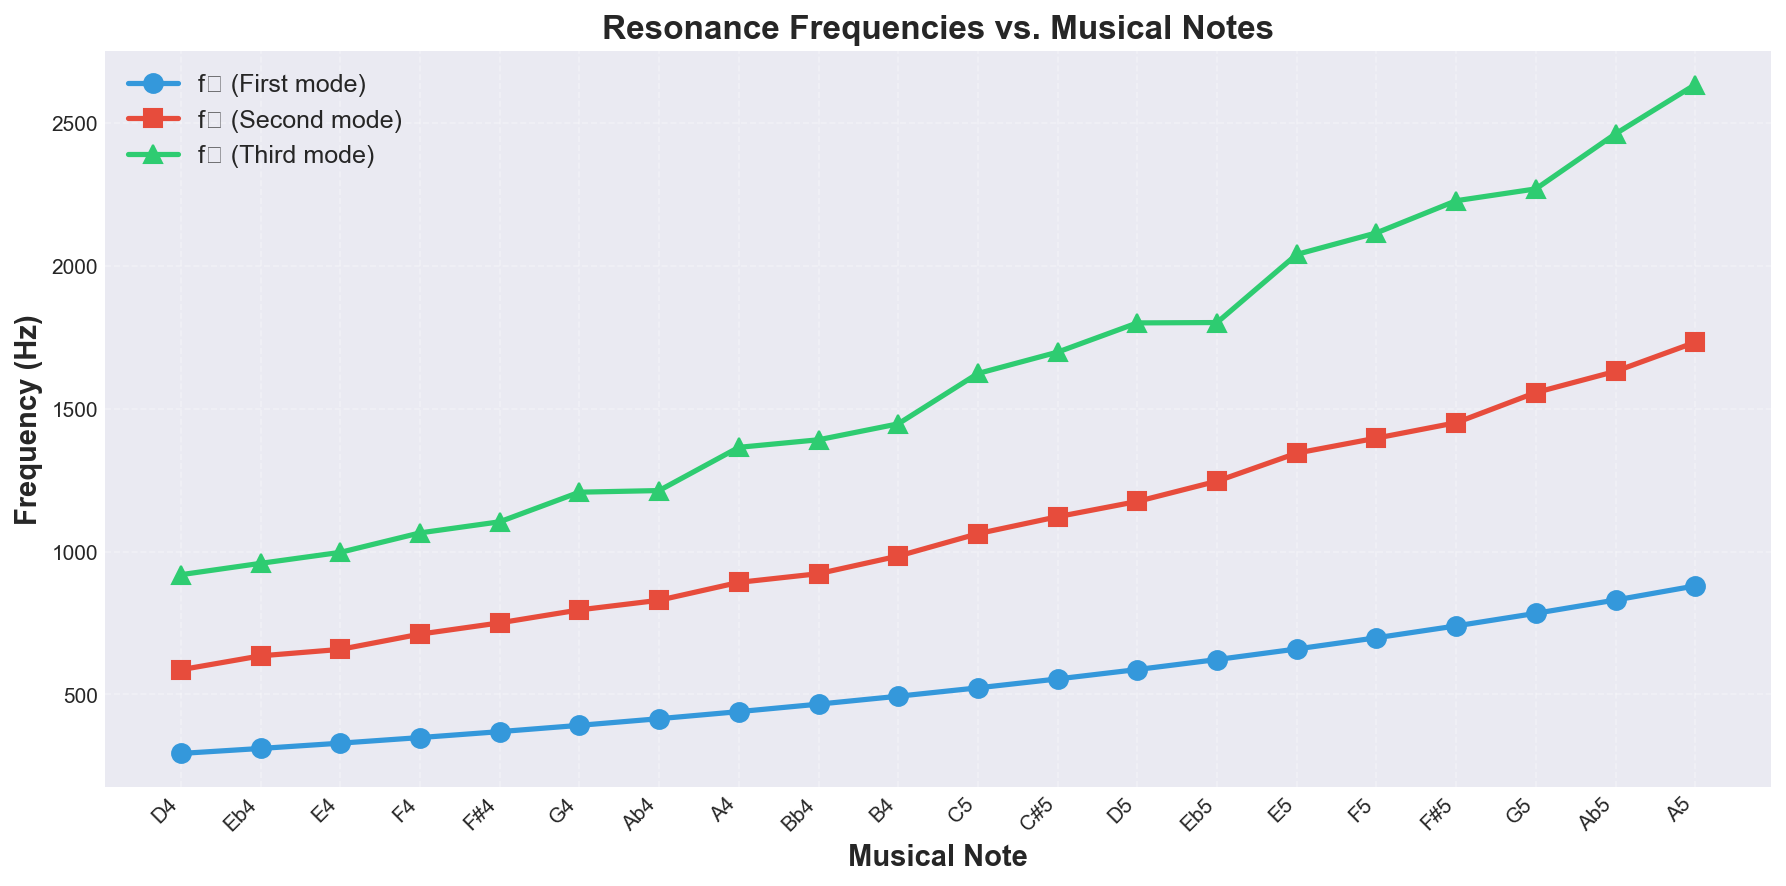
\includegraphics[width=0.7\textwidth]{presentation_screenshots/screenshot_resonance_frequencies.png}
\end{figure}
\end{frame}

\begin{frame}{Inharmonicity}
\textbf{Definition:}
\begin{equation*}
\Delta = 1200 \log_2\left(\frac{f_{\text{play}}}{f_0}\right) \quad \text{[cents]}
\end{equation*}

where:
\begin{itemize}
    \item $f_{\text{play}}$: Target playing frequency (from fingering chart)
    \item $f_0$: First antiresonance frequency (impedance minimum)
\end{itemize}

\textbf{Interpretation:}
\begin{itemize}
    \item $\Delta \approx 0$: Well-tuned note
    \item $\Delta > 0$: Note is sharp (player must flatten)
    \item $\Delta < 0$: Note is flat (player must sharpen)
\end{itemize}

\textbf{Physical Significance:} Quantifies the intonation adjustment required relative to the instrument's passive resonance

\begin{figure}
\centering
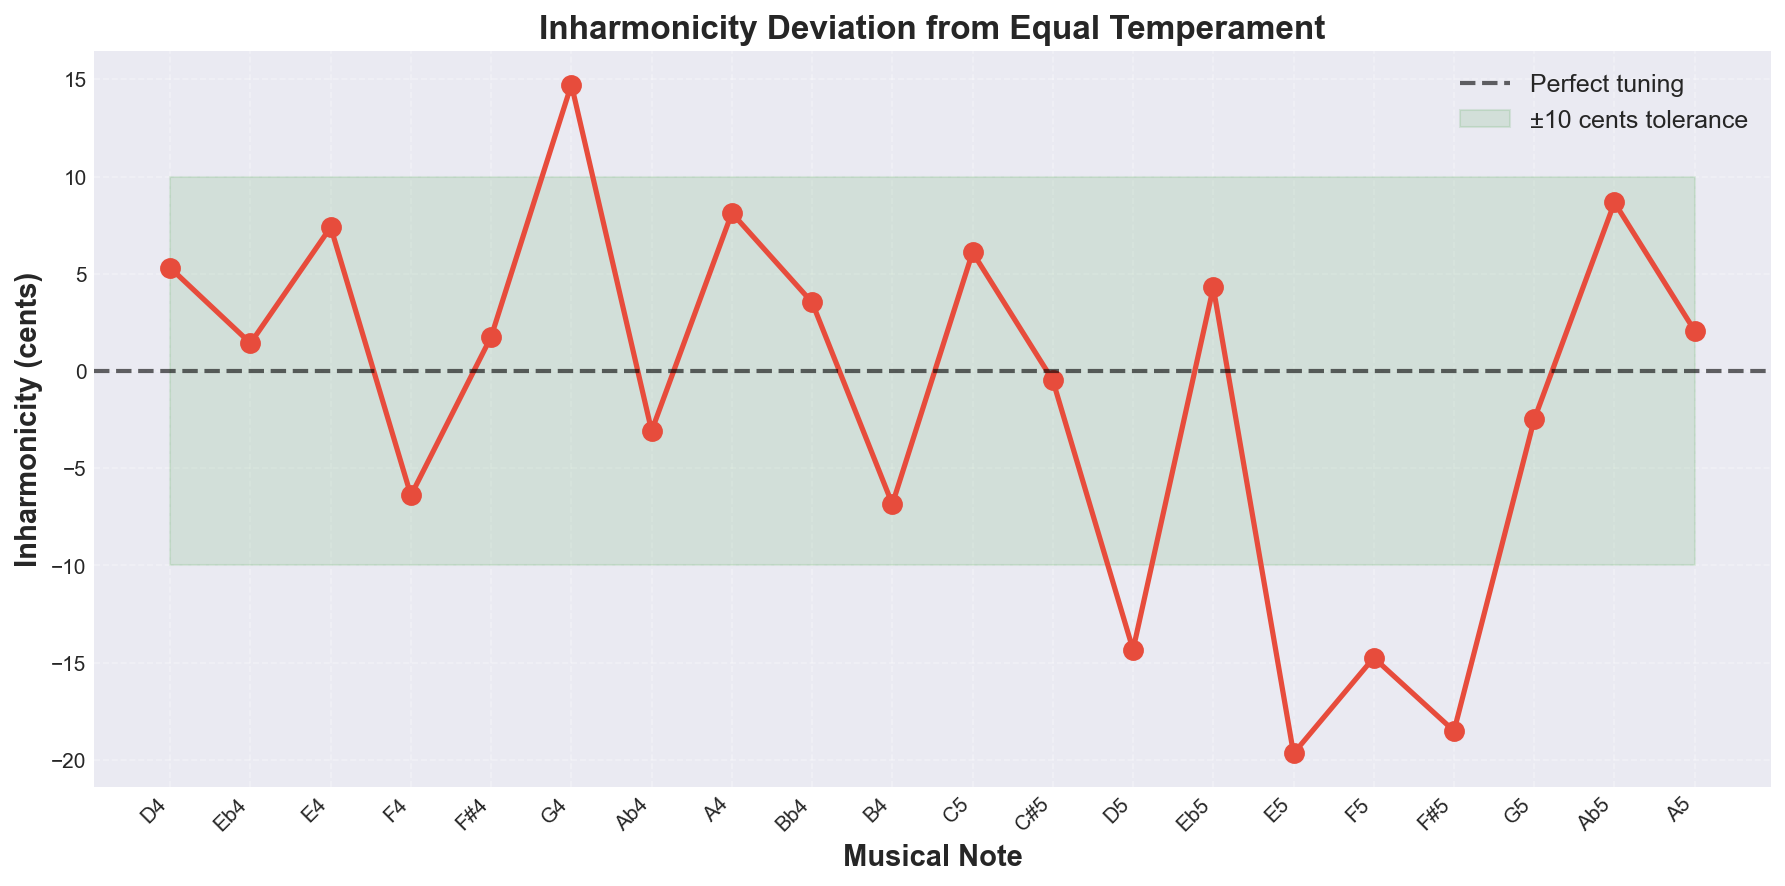
\includegraphics[width=0.7\textwidth]{presentation_screenshots/screenshot_inharmonicity.png}
\end{figure}
\end{frame}

\begin{frame}{Mouthpiece Octave Compensation (MOC)}
\textbf{Physical Basis:}
Frequency-dependent embouchure end correction:
\begin{equation*}
L_{\text{eff},n} = L + \Delta L_{\text{head},n} + \Delta L_{\text{foot},n}
\end{equation*}

Headjoint cavity impedance:
\begin{equation*}
Z_{\text{cav}}(f) = -jZ_0 \cot(kL_h)
\end{equation*}

where $k = 2\pi f/c$ and $L_h$ is the headjoint cavity length.

\textbf{Octave Ratio:}
\begin{equation*}
\frac{f_{\text{II}}}{2f_{\text{I}}} = \frac{L_{\text{eff},1}}{L_{\text{eff},2}} = \frac{L + \Delta L_{\text{head},1}}{L + \Delta L_{\text{head},2}}
\end{equation*}

Typically: $\Delta L_{\text{head},1} > \Delta L_{\text{head},2}$ (second mode sharp relative to octave)
\end{frame}

\begin{frame}{MOC Metrics}
\textbf{Embouchure Length Corrections:}
\begin{equation*}
\Delta l_n = \frac{c}{4}\left(\frac{1}{f_{\text{res},n}} - \frac{1}{f_{\text{play},n}}\right)
\end{equation*}

\textbf{MOC Difference:}
\begin{equation*}
\text{MOC}_\Delta = \Delta l_{\text{I}} - \Delta l_{\text{II}} = \frac{c}{4}\left(\frac{1}{f_{\text{res},1}} - \frac{2}{f_{\text{play}}}\right)
\end{equation*}

\textbf{MOC Ratio:}
\begin{equation*}
\text{MOC}_R = \frac{\Delta l_{\text{I}}}{\Delta l_{\text{II}}} = \frac{1 - \frac{f_{\text{res},1}}{f_{\text{play}}}}{1 - \frac{f_{\text{res},2}}{2f_{\text{play}}}}
\end{equation*}

\textbf{Displayed Metric:}
\begin{equation*}
\text{MOC} = \frac{f_1 - f_0}{f_{\text{play,II}} - f_{\text{play,I}}}
\end{equation*}

\begin{figure}
\centering
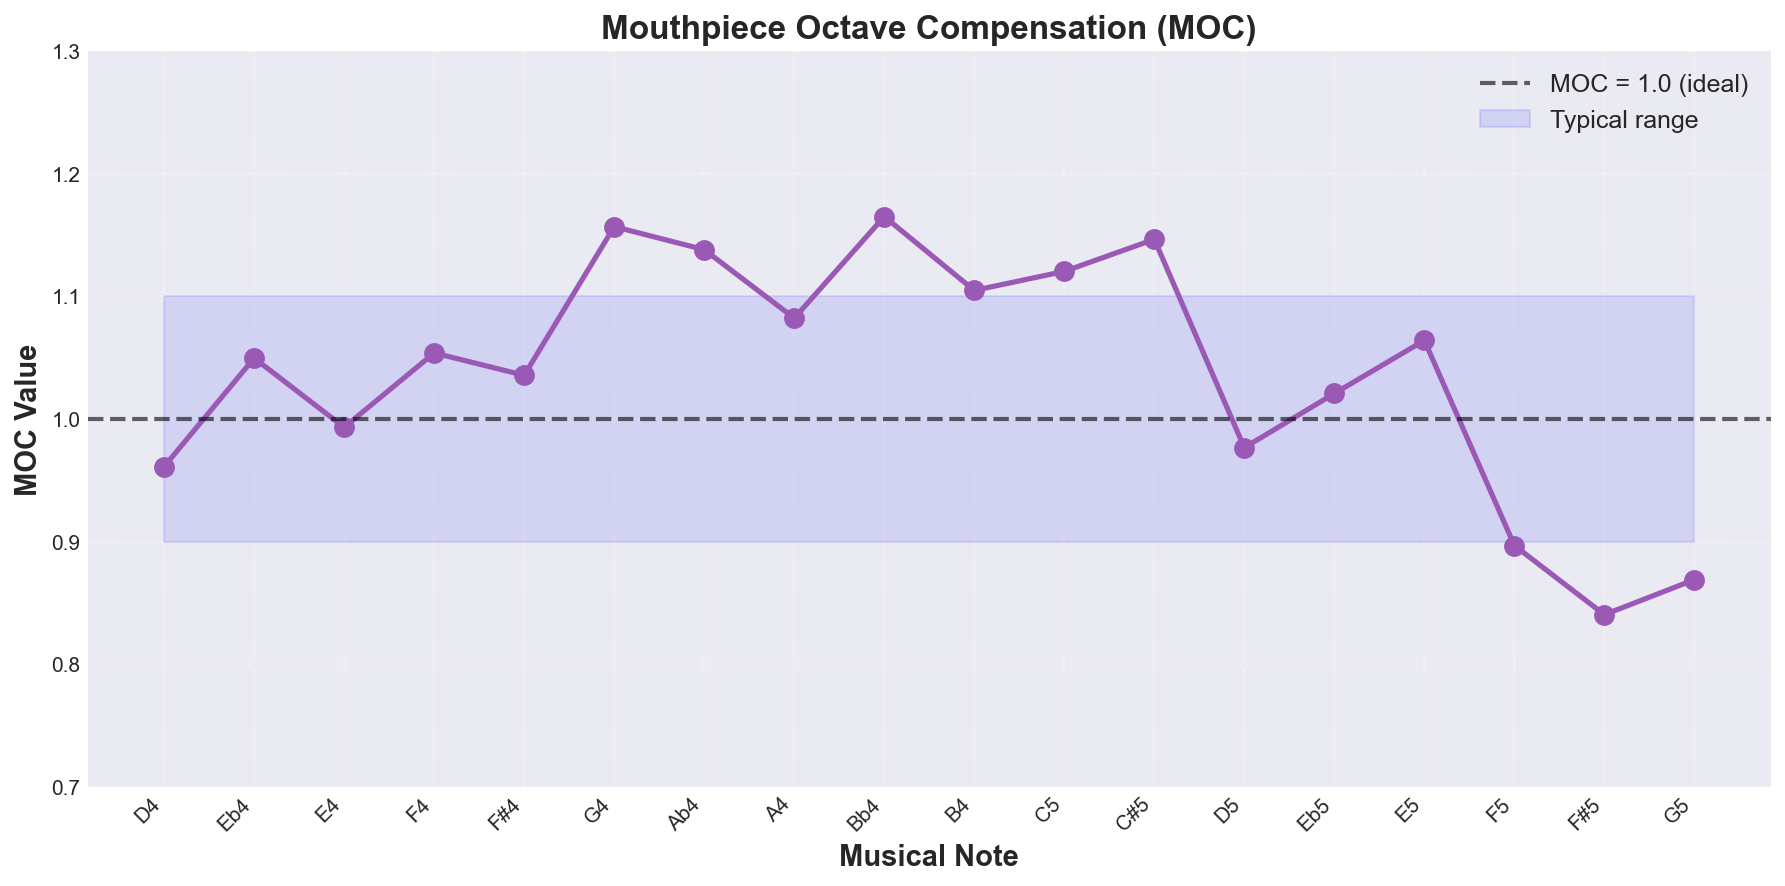
\includegraphics[width=0.7\textwidth]{presentation_screenshots/screenshot_moc.png}
\end{figure}
\end{frame}

\begin{frame}{First-Octave Pitch Adjustment ($B_I$)}
\textbf{Definition:}
\begin{equation*}
B_I = 1200 \log_2\left(\frac{f_{\text{play,I}}}{f_0}\right) \quad \text{[cents]}
\end{equation*}

\textbf{Physical Interpretation:}
\begin{itemize}
    \item $B_I > 0$: Player needs to play sharper than passive $f_0$
    \item $B_I < 0$: Player needs to play flatter than passive $f_0$
    \item $B_I \approx 0$: Passive $f_0$ is already close to target pitch
\end{itemize}

\textbf{Significance:} Directly reflects the basic intonation challenge presented by the instrument for each note in the first register.

\begin{figure}
\centering
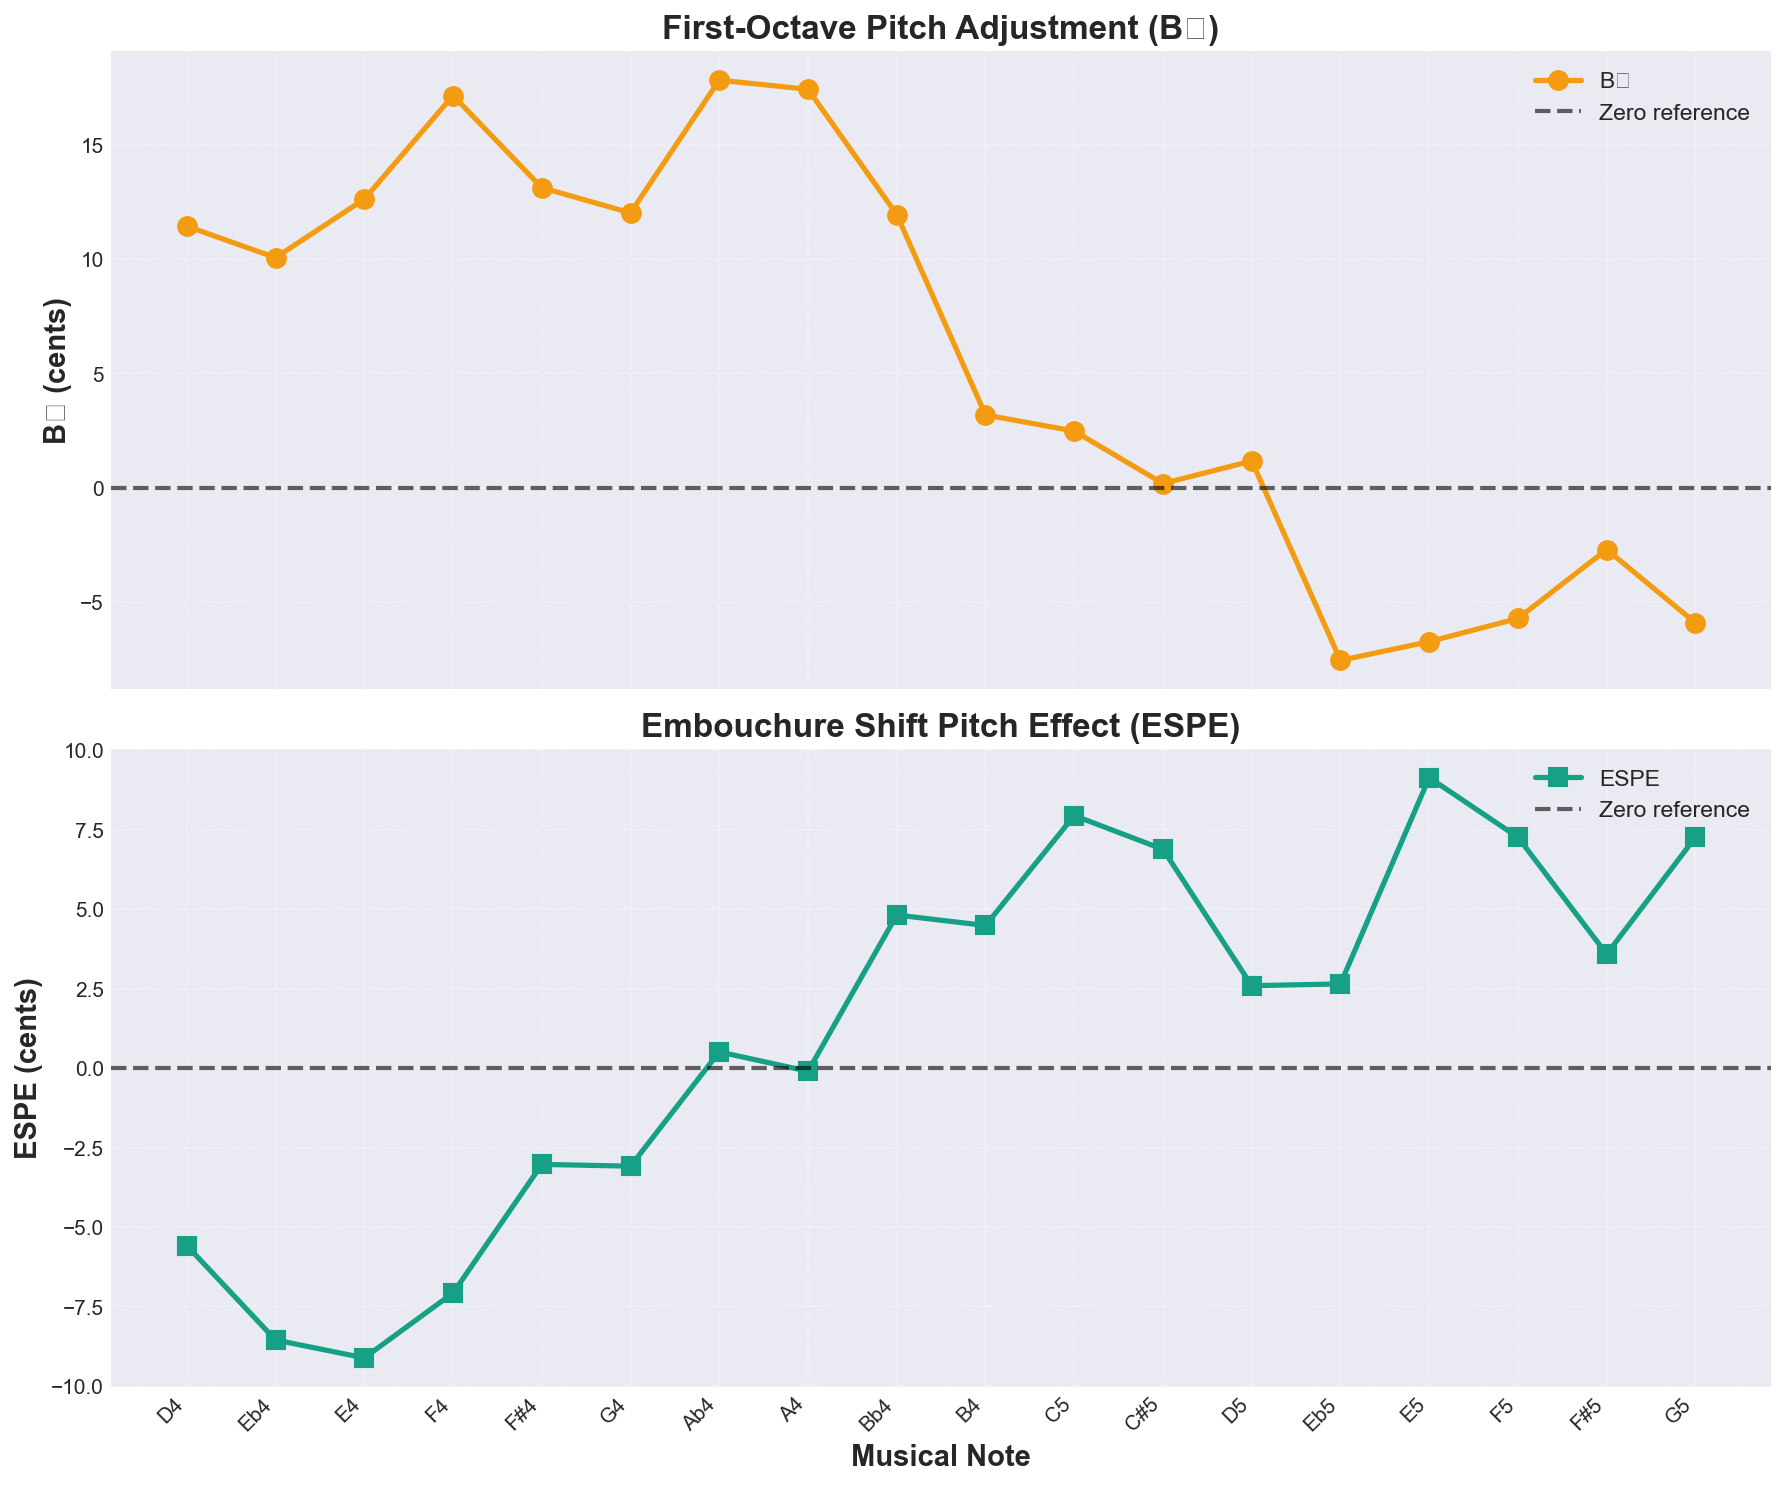
\includegraphics[width=0.7\textwidth]{presentation_screenshots/screenshot_bi_espe.png}
\end{figure}
\end{frame}

\begin{frame}{Embouchure Shift Pitch Effect (ESPE)}
\textbf{Embouchure Corrections:}
\begin{align*}
\Delta l_{\text{emb},n} &\approx \frac{nc}{2}\left(\frac{1}{f_{\text{play},n}} - \frac{1}{f_n}\right) \\
\Delta l_{\text{I,emb}} &= \frac{c}{2}\left(\frac{1}{f_{\text{play,I}}} - \frac{1}{f_0}\right) \\
\Delta l_{\text{II,emb}} &= c\left(\frac{1}{f_{\text{play,II}}} - \frac{1}{f_1}\right)
\end{align*}

\textbf{Differential Correction:}
\begin{equation*}
\Delta(\Delta l_{\text{emb}}) = \Delta l_{\text{II,emb}} - \Delta l_{\text{I,emb}}
\end{equation*}

\textbf{ESPE:}
\begin{equation*}
\text{ESPE} = 1200 \log_2\left(\frac{L_{\text{eff,I}}}{L_{\text{eff,I}} + \Delta(\Delta l_{\text{emb}})}\right) \quad \text{[cents]}
\end{equation*}

\textbf{Interpretation:} Estimates the pitch change induced on the fundamental by the differential embouchure correction required for the octave jump.

\vspace{-0.5cm}
\end{frame}

\begin{frame}{Q-Factor}
\textbf{Definition:}
\begin{equation*}
Q = \frac{f_0}{\Delta f}
\end{equation*}

where $\Delta f$ is the bandwidth at -3 dB from the peak admittance.

\textbf{Calculation:}
\begin{itemize}
    \item Find peak admittance: $|Y|_{\text{max}}$ at $f_0$
    \item Calculate threshold: $|Y|_{\text{threshold}} = |Y|_{\text{max}} / \sqrt{2}$
    \item Find frequencies where $|Y| = |Y|_{\text{threshold}}$: $f_{\text{left}}$, $f_{\text{right}}$
    \item Bandwidth: $\Delta f = f_{\text{right}} - f_{\text{left}}$
\end{itemize}

\textbf{Physical Significance:}
\begin{itemize}
    \item Higher $Q$: Sharper resonance, better mode isolation
    \item Lower $Q$: Broader resonance, more damping
\end{itemize}

\begin{figure}
\centering
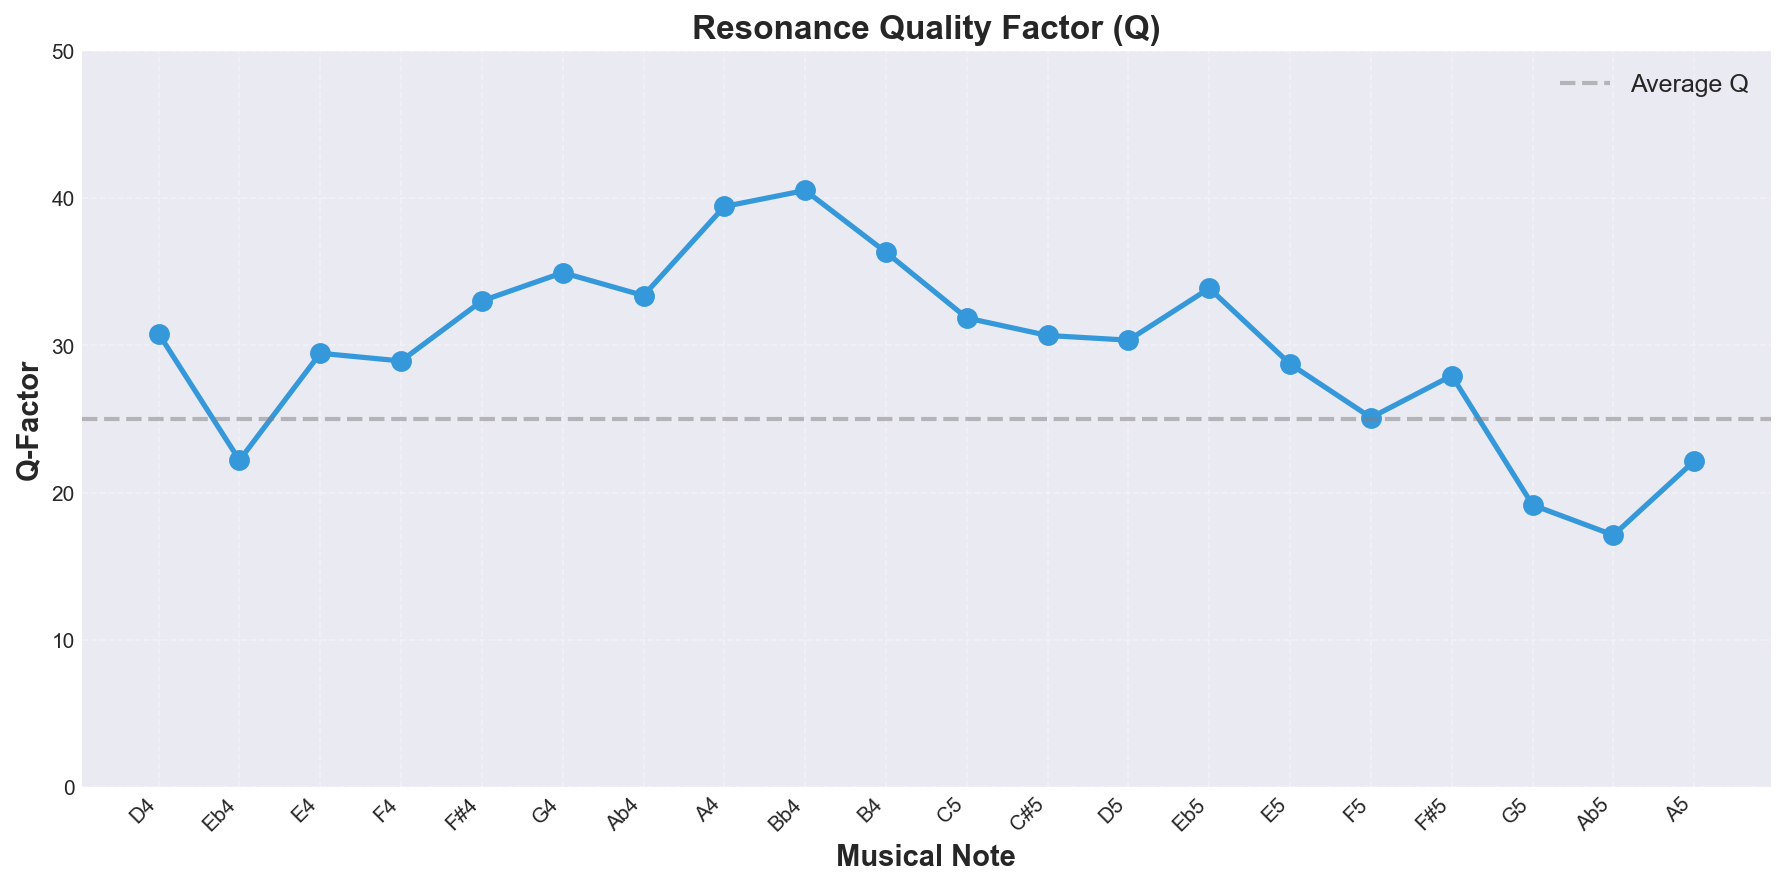
\includegraphics[width=0.7\textwidth]{presentation_screenshots/screenshot_qfactor.png}
\end{figure}
\end{frame}

\begin{frame}{Harmonic Ratios}
\textbf{Definition:}
\begin{align*}
\text{Ratio}_{f_1/f_0} &= \frac{f_1}{f_0} \\
\text{Ratio}_{f_2/f_0} &= \frac{f_2}{f_0} \\
\text{Ratio}_{f_2/f_1} &= \frac{f_2}{f_1}
\end{align*}

\textbf{Ideal Values (Perfect Harmonic Series):}
\begin{itemize}
    \item $f_1/f_0 = 2.0$ (octave)
    \item $f_2/f_0 = 3.0$ (twelfth)
    \item $f_2/f_1 = 1.5$ (perfect fifth)
\end{itemize}

\textbf{Deviations indicate:}
\begin{itemize}
    \item Bore conicity effects
    \item End correction frequency dependence
    \item Hole interaction effects
\end{itemize}

\begin{figure}
\centering
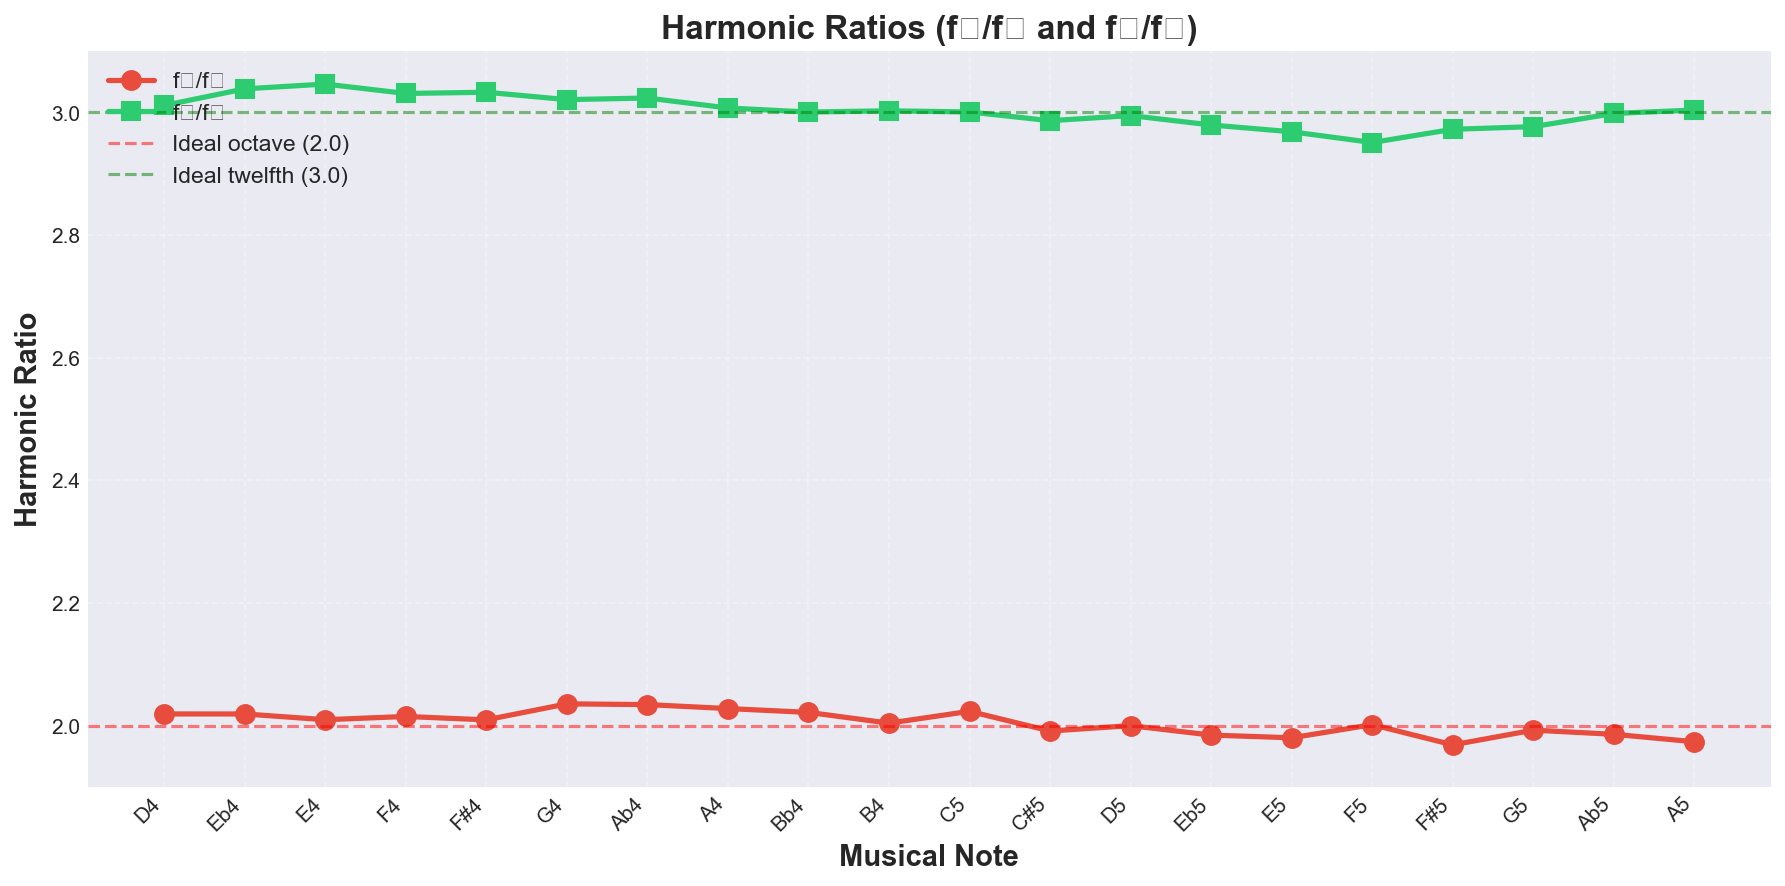
\includegraphics[width=0.7\textwidth]{presentation_screenshots/screenshot_harmonic_ratios.png}
\end{figure}
\end{frame}

\begin{frame}{Peak Heights and Tonal Characteristics}
\textbf{Admittance Peak Heights:}
\begin{equation*}
|Y|_{\text{dB}} = 20 \log_{10}(|Y|) \quad \text{[dB]}
\end{equation*}

\textbf{Significance:}
\begin{itemize}
    \item Higher peaks: Stronger resonance, easier to excite
    \item Lower peaks: Weaker resonance, requires more player effort
\end{itemize}

\textbf{Tonal Characteristics:}
\begin{itemize}
    \item Mode coupling strength
    \item Register transition ease
    \item Timbre quality indicators
\end{itemize}

\begin{figure}
\centering
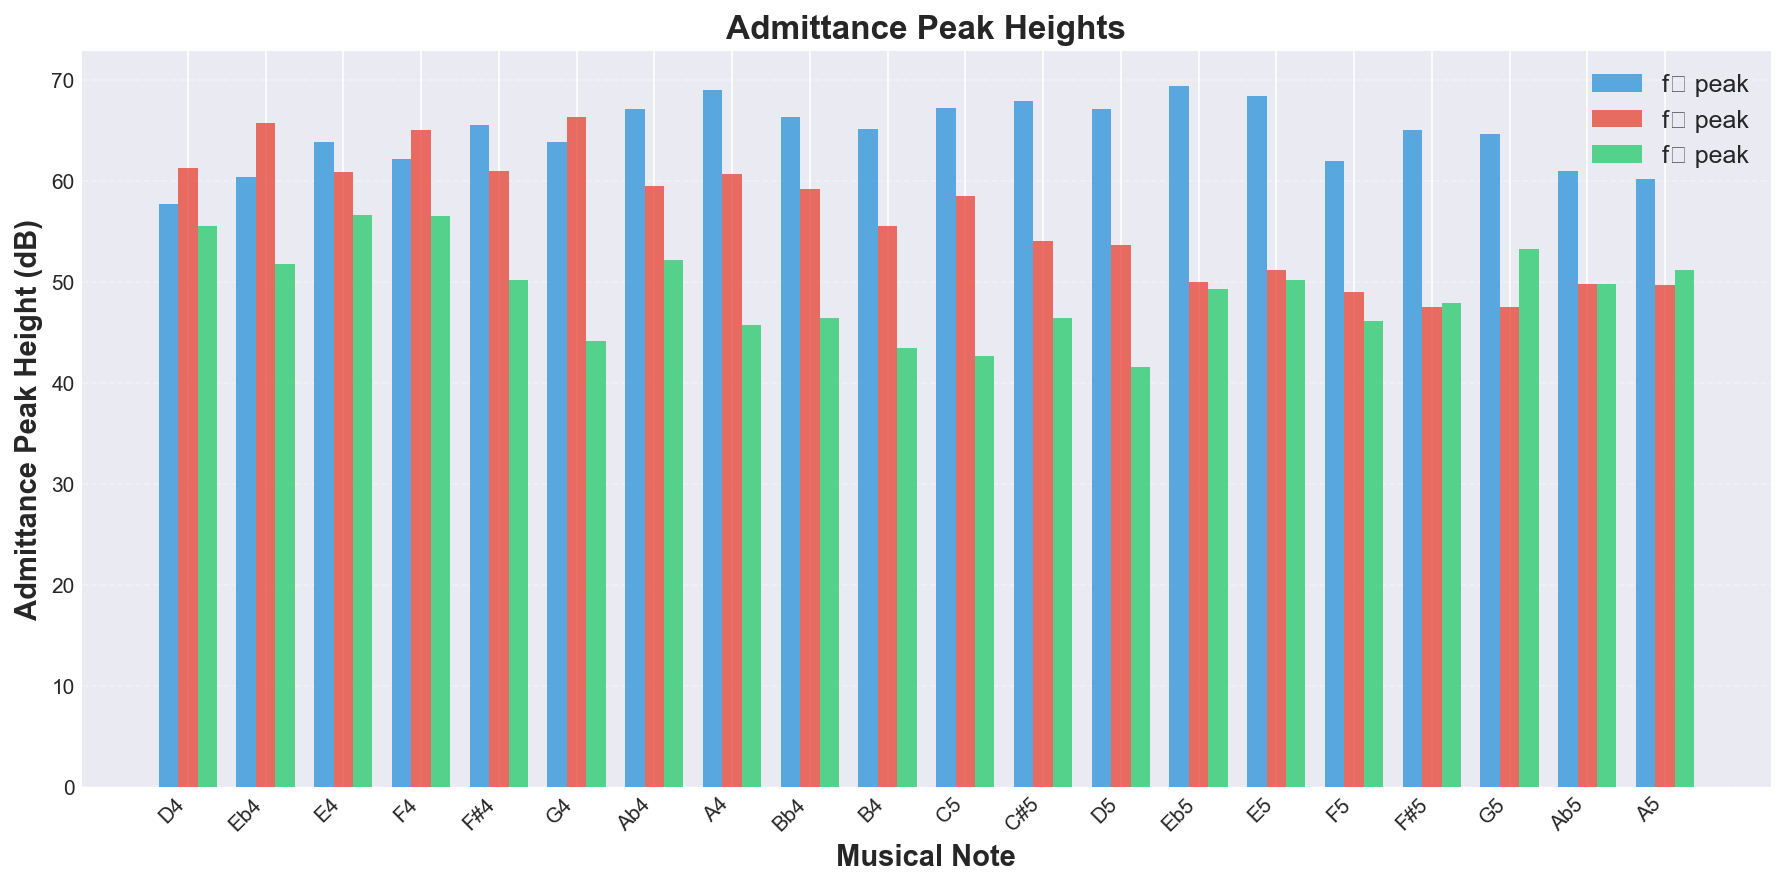
\includegraphics[width=0.7\textwidth]{presentation_screenshots/screenshot_peak_heights.png}
\end{figure}
\end{frame}

% ==================== SECTION 4: RESONATOR TRUNCATION ANALYSIS ====================
\section{Resonator Truncation Analysis}

\begin{frame}{Novel Analysis Method}
\textbf{Concept:}
\begin{itemize}
    \item Analyze the acoustic response of the \textbf{bore alone} (without holes)
    \item Progressively truncate the geometry from the end
    \item Study how length and conicity affect resonance frequencies
\end{itemize}

\textbf{Advantages:}
\begin{itemize}
    \item \textbf{Isolates pure geometry effects}: No hole interference
    \item \textbf{Reveals length-frequency relationships}: Direct observation of how truncation affects modes
    \item \textbf{Acoustically valid}: Similar to "cutoff length" studies in wind instrument acoustics
\end{itemize}

\textbf{Method:}
\begin{enumerate}
    \item Truncate geometry to percentage of total length (100\%, 95\%, 90\%, \ldots, 20\%)
    \item Calculate impedance for each truncated section
    \item Extract acoustic metrics for each length
    \item Visualize trends vs. truncated length
\end{enumerate}
\end{frame}

\begin{frame}{Truncation Geometry}
\textbf{Process:}
\begin{itemize}
    \item Maintain cork position at $x = 0$
    \item Truncate from the end (foot side)
    \item Interpolate diameter at truncation point if needed
    \item Ensure minimum length (default: 50 mm)
\end{itemize}

\textbf{OpenWind Configuration:}
\begin{itemize}
    \item No side holes (except optionally embouchure)
    \item Dummy fingering chart (all holes "open")
    \item Source location: "entrance" (embouchure)
    \item Open end radiation: unflanged
\end{itemize}

\textbf{Effective Length:}
\begin{equation*}
L_{\text{truncated}} = L_{\text{total}} \times \frac{\text{percentage}}{100}
\end{equation*}
\end{frame}

\begin{frame}{Resonator Truncation Metrics}
For each truncated length, we calculate:

\begin{enumerate}
    \item \textbf{Resonance Frequencies:} $f_0, f_1, f_2, \ldots$
    \begin{equation*}
    f_n = \arg\min_f |Z(f)|
    \end{equation*}
    
    \item \textbf{Inharmonicity:}
    \begin{equation*}
    \Delta_{\text{cents}} = 1200 \log_2\left(\frac{f_1}{2f_0}\right)
    \end{equation*}
    
    \item \textbf{Harmonic Ratios:}
    \begin{align*}
    \frac{f_1}{f_0}, \quad \frac{f_2}{f_0}, \quad \frac{f_2}{f_1}
    \end{align*}
    
    \item \textbf{Effective Length:}
    \begin{equation*}
    L_{\text{eff}} = \frac{c}{2f_0}
    \end{equation*}
    
    \item \textbf{Q-Factor:} For each mode
\end{enumerate}
\end{frame}

\begin{frame}{Resonator Truncation Visualizations}
\textbf{Four Main Plots:}

\begin{enumerate}
    \item \textbf{Resonance Frequencies vs. Length}
    \begin{itemize}
        \item Shows how $f_0, f_1, f_2$ change with truncation
        \item Reveals conicity effects on mode spacing
    \end{itemize}
    
    \item \textbf{Inharmonicity vs. Length}
    \begin{itemize}
        \item Quantifies deviation from perfect harmonic series
        \item Shows how geometry affects octave tuning
    \end{itemize}
    
    \item \textbf{Harmonic Ratios vs. Length}
    \begin{itemize}
        \item $f_1/f_0$ and $f_2/f_0$ with ideal reference lines
        \item Reveals mode coupling and conicity effects
    \end{itemize}
    
    \item \textbf{Impedance Curves Overlay}
    \begin{itemize}
        \item Superimposed impedance magnitude for different lengths
        \item Shows frequency shift and peak broadening
    \end{itemize}
\end{enumerate}

\vspace{0.3cm}
\textbf{Note:} See dedicated slides below for individual plots.
\end{frame}

\begin{frame}{Resonator Truncation: Frequencies vs. Length}
\begin{figure}
\centering
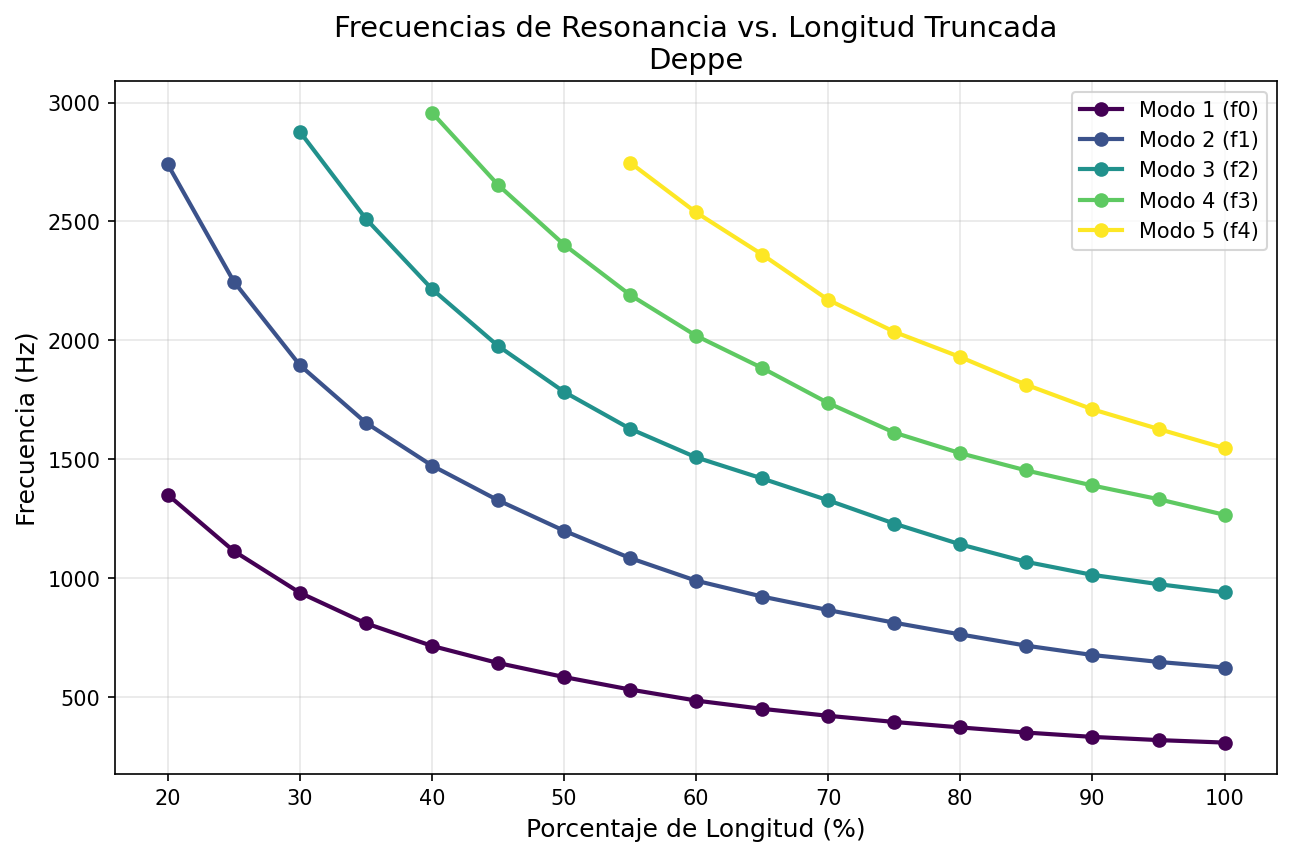
\includegraphics[width=0.75\textwidth]{presentation_screenshots/resonator_truncation_frequencies.png}
\end{figure}
\vspace{-0.3cm}
\begin{itemize}
    \item Shows how fundamental and overtone frequencies change with truncation
    \item Reveals conicity effects on mode spacing
\end{itemize}
\end{frame}

\begin{frame}{Resonator Truncation: Inharmonicity vs. Length}
\begin{figure}
\centering
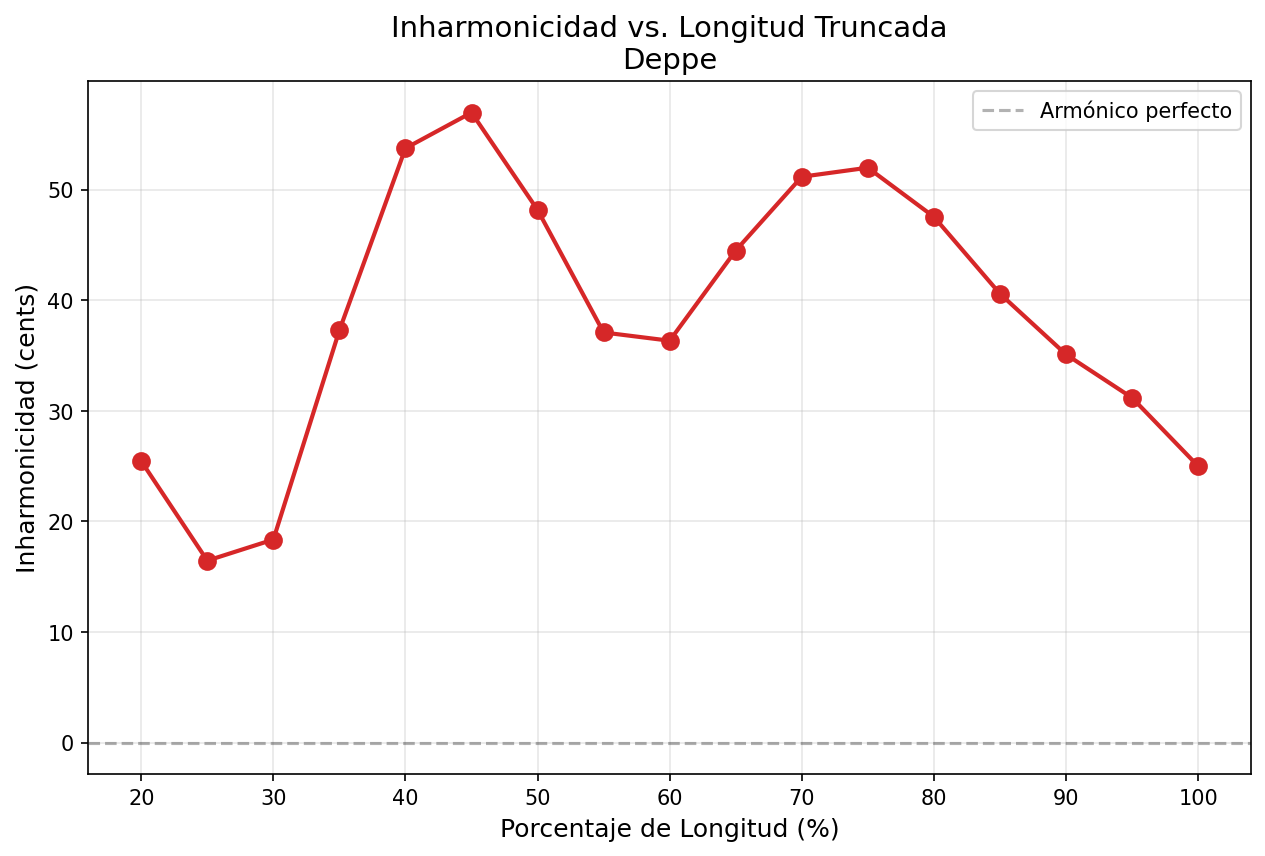
\includegraphics[width=0.75\textwidth]{presentation_screenshots/resonator_truncation_inharmonicity.png}
\end{figure}
\vspace{-0.3cm}
\begin{itemize}
    \item Quantifies deviation from perfect harmonic series
    \item Demonstrates geometry impact on octave tuning
\end{itemize}
\end{frame}

\begin{frame}{Resonator Truncation: Harmonic Ratios vs. Length}
\begin{figure}
\centering
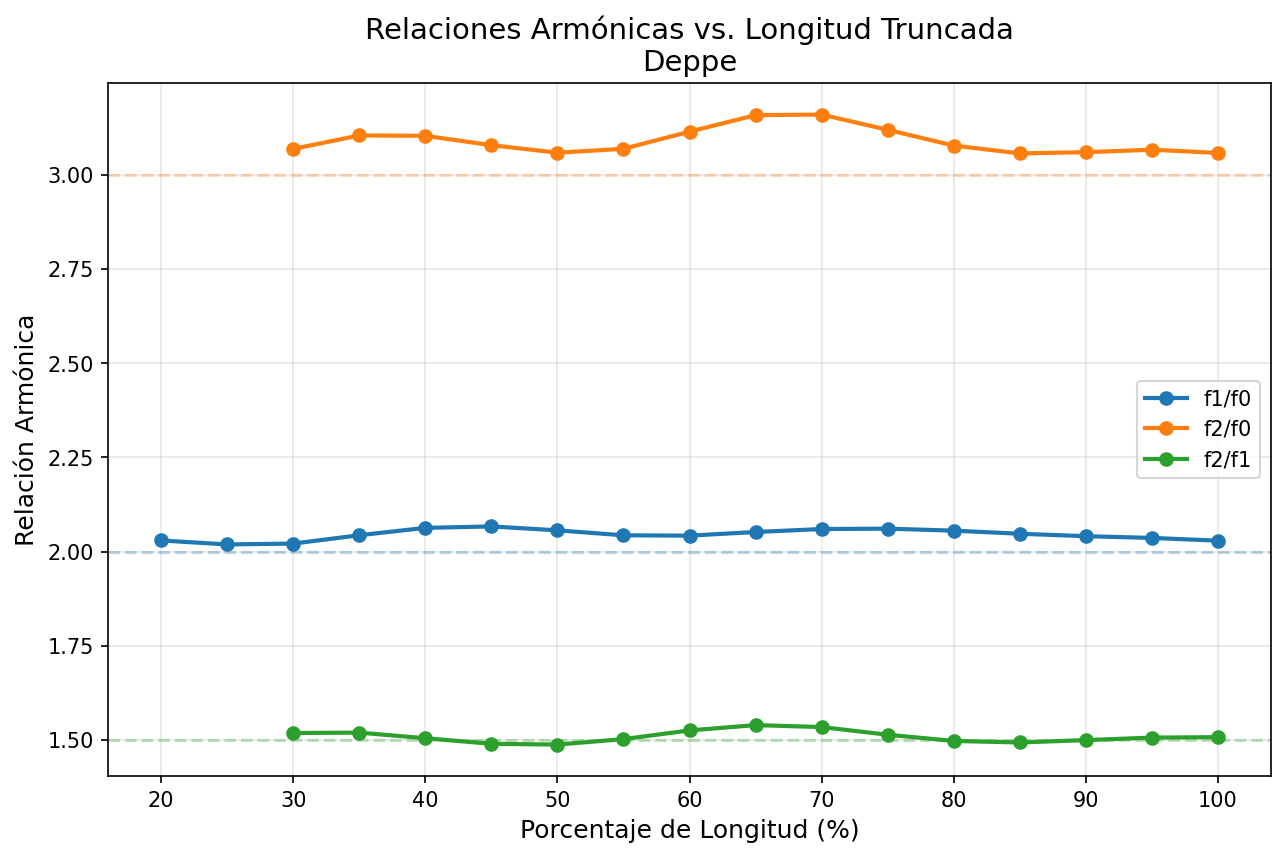
\includegraphics[width=0.75\textwidth]{presentation_screenshots/resonator_truncation_harmonic_ratios.png}
\end{figure}
\vspace{-0.3cm}
\begin{itemize}
    \item Compares $f_1/f_0$ and $f_2/f_0$ ratios to ideal values
    \item Shows mode coupling and conicity effects
\end{itemize}
\end{frame}

\begin{frame}{Resonator Truncation: Impedance Overlay}
\begin{figure}
\centering
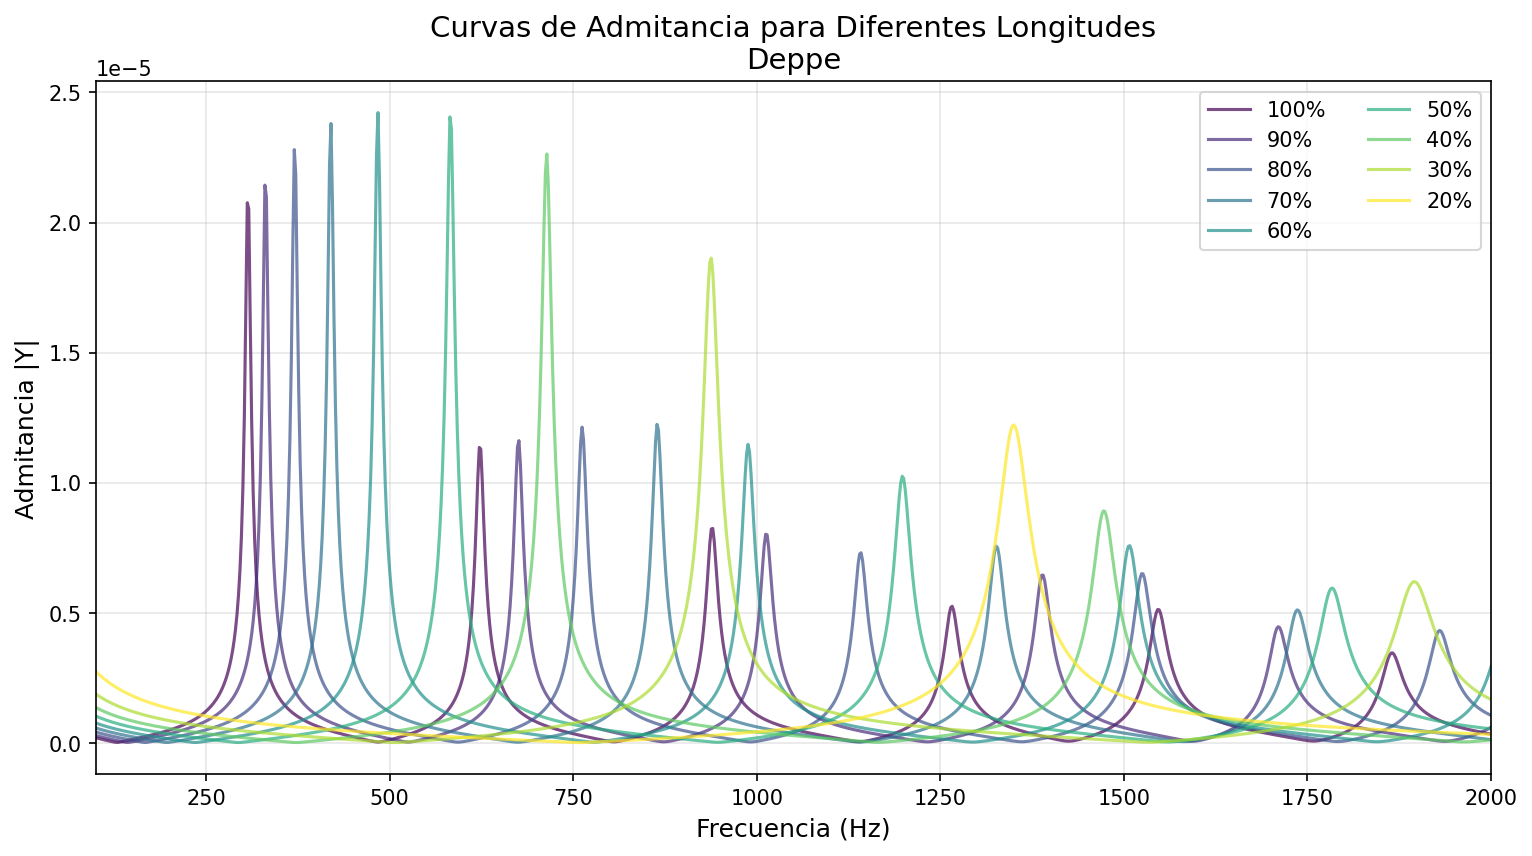
\includegraphics[width=0.75\textwidth]{presentation_screenshots/resonator_truncation_impedance_overlay.png}
\end{figure}
\vspace{-0.3cm}
\begin{itemize}
    \item Superimposed impedance curves for different truncated lengths
    \item Visualizes frequency shift and peak broadening with length reduction
\end{itemize}
\end{frame}

\begin{frame}{Resonator Truncation: Physical Interpretation}
\textbf{Key Observations:}

\begin{itemize}
    \item \textbf{Length-Frequency Relationship:}
    \begin{equation*}
    f_n \propto \frac{1}{L_{\text{truncated}}}
    \end{equation*}
    As length decreases, frequencies increase.
    
    \item \textbf{Conicity Effects:}
    \begin{itemize}
        \item Tapered bores show non-linear frequency shifts
        \item Mode spacing deviates from harmonic series
        \item Truncation reveals local vs. global geometry effects
    \end{itemize}
    
    \item \textbf{End Correction:}
    \begin{itemize}
        \item Effective length includes end corrections
        \item Truncation point acts as new open end
        \item Correction depends on truncation diameter
    \end{itemize}
\end{itemize}

\textbf{Applications:}
\begin{itemize}
    \item Design optimization for specific frequency ranges
    \item Understanding bore geometry influence
    \item Comparative analysis across different flutes
\end{itemize}
\end{frame}

% ==================== SECTION 5: SENSITIVITY ANALYSIS ====================
\section{Sensitivity Analysis}

\begin{frame}{Parameter Variation Studies}
\textbf{Concept:}
Systematically vary geometric parameters and observe acoustic response changes.

\textbf{Available Parameters:}

\begin{enumerate}
    \item \textbf{Hole Undercut Angle} (Priority 1)
    \begin{itemize}
        \item Modifies conical hole geometry
        \item Range: 0° (cylindrical) to 15° (strong undercut)
        \item Affects: Intonation, register response
    \end{itemize}
    
    \item \textbf{Part Taper Angle} (Priority 2)
    \begin{itemize}
        \item Modifies bore conicity of individual parts
        \item Affects: Overall bore profile, mode spacing
    \end{itemize}
    
    \item \textbf{Wall Thickness} (Priority 3)
    \begin{itemize}
        \item Constant, variable, or proportional profiles
        \item Affects: External geometry, mass distribution
    \end{itemize}
\end{enumerate}
\end{frame}

\begin{frame}{Sensitivity Analysis Workflow}
\textbf{Process:}

\begin{enumerate}
    \item \textbf{Select Base Flute:} Choose reference instrument
    \item \textbf{Choose Parameter:} Select geometric parameter to vary
    \item \textbf{Define Range:} Set min, max, and step values
    \item \textbf{Generate Variants:} System creates geometric variants
    \item \textbf{Calculate Acoustic Response:} Full impedance analysis for each variant
    \item \textbf{Extract Metrics:} Compute all acoustic metrics
    \item \textbf{Visualize Results:} Parameter vs. metric plots
    \item \textbf{Generate Report:} Comprehensive PDF report
\end{enumerate}

\textbf{Output:}
\begin{itemize}
    \item Sensitivity plots (parameter vs. acoustic metrics)
    \item Complete acoustic analysis for all variants
    \item Statistical summaries
    \item Design recommendations
\end{itemize}

\vspace{0.3cm}
\textit{Interactive dialog for parameter selection and range specification}
\end{frame}

\begin{frame}{Sensitivity Analysis: Example Results}
\textbf{Typical Outputs:}

\begin{itemize}
    \item \textbf{Parameter Sweep Plots:}
    \begin{itemize}
        \item Undercut angle vs. inharmonicity
        \item Undercut angle vs. MOC
        \item Undercut angle vs. $B_I$ and ESPE
    \end{itemize}
    
    \item \textbf{Optimal Range Identification:}
    \begin{itemize}
        \item Parameter values minimizing inharmonicity
        \item Values achieving target MOC
        \item Trade-offs between different metrics
    \end{itemize}
    
    \item \textbf{Design Insights:}
    \begin{itemize}
        \item Critical parameters requiring precision
        \item Tolerant parameters with wide acceptable ranges
        \item Interaction effects between parameters
    \end{itemize}
\end{itemize}

\vspace{0.3cm}
\textit{Example plots showing undercut angle vs. inharmonicity, MOC, etc.}
\end{frame}

% ==================== SECTION 6: DATABASE AND STATISTICS ====================
\section{Database \& Statistics}

\begin{frame}{Database Architecture}
\textbf{SQLite Database Structure:}

\begin{itemize}
    \item \textbf{Flutes Table:} General information, metadata
    \item \textbf{Flute Geometry:} Internal geometry per part (JSON)
    \item \textbf{External Geometry:} External profiles (measured/parametric)
    \item \textbf{Impedance Calculation Params:} Calculation parameters (hash-based)
    \item \textbf{Impedance Results:} Cached impedance computations
    \item \textbf{Bore Geometry:} OpenWind-compatible geometry
    \item \textbf{Side Holes:} Hole definitions for OpenWind
\end{itemize}

\textbf{Benefits:}
\begin{itemize}
    \item Fast retrieval of previous calculations
    \item Parameter change detection
    \item Efficient storage of large impedance datasets
    \item Multi-flute comparison capabilities
\end{itemize}
\end{frame}

\begin{frame}{Statistical Reporting}
\textbf{Comprehensive Database Reports:}

\begin{enumerate}
    \item \textbf{Geometric Statistics:}
    \begin{itemize}
        \item Bore diameter distributions
        \item Hole size statistics
        \item Length measurements
        \item Conicity analysis
    \end{itemize}
    
    \item \textbf{Acoustic Statistics:}
    \begin{itemize}
        \item Inharmonicity distributions
        \item MOC statistics across flutes
        \item $B_I$ and ESPE ranges
        \item Q-factor distributions
    \end{itemize}
    
    \item \textbf{Comparative Analysis:}
    \begin{itemize}
        \item Flute-to-flute comparisons
        \item Historical period analysis
        \item Maker-specific characteristics
    \end{itemize}
    
    \item \textbf{Visualizations:}
    \begin{itemize}
        \item Histograms, box plots, scatter plots
        \item Correlation matrices
        \item Multi-flute overlays
    \end{itemize}
\end{enumerate}

\vspace{0.3cm}
\textit{Comprehensive PDF reports with histograms, distributions, and correlations}
\end{frame}

% ==================== SECTION 7: ENGINEERING TOOLS ====================
\section{Engineering Tools}

\begin{frame}{Engineering Drawings}
\textbf{Automated PDF Generation:}

\begin{itemize}
    \item \textbf{Technical Drawings:}
    \begin{itemize}
        \item Multi-view projections
        \item Dimensioned drawings
        \item Cross-sections
        \item Hole detail views
    \end{itemize}
    
    \item \textbf{Geometric Accuracy:}
    \begin{itemize}
        \item Scale-accurate representations
        \item Proper dimensioning
        \item Manufacturing-ready format
    \end{itemize}
    
    \item \textbf{Customization:}
    \begin{itemize}
        \item Select parts to include
        \item Choose views
        \item Add annotations
    \end{itemize}
\end{itemize}

\vspace{0.3cm}
\textit{Automated technical drawings with dimensions and cross-sections}
\end{frame}

\begin{frame}{G-Code Generation}
\textbf{CNC Manufacturing Support:}

\begin{itemize}
    \item \textbf{Automatic G-Code Generation:}
    \begin{itemize}
        \item Toolpath generation for bore machining
        \item Hole drilling sequences
        \item Multi-axis support
    \end{itemize}
    
    \item \textbf{Parameters:}
    \begin{itemize}
        \item Tool diameter and type
        \item Feed rates and speeds
        \item Depth of cut
        \item Safety clearances
    \end{itemize}
    
    \item \textbf{Output:}
    \begin{itemize}
        \item Standard G-code format
        \item Compatible with common CNC controllers
        \item Validation and simulation support
    \end{itemize}
\end{itemize}

\vspace{0.3cm}
\textit{CNC toolpath generation with configurable parameters}
\end{frame}

\begin{frame}{Interactive Geometry Editor}
\textbf{Features:}

\begin{itemize}
    \item \textbf{Visual Editing:}
    \begin{itemize}
        \item Click-and-drag hole positions
        \item Adjust diameters interactively
        \item Modify measurements in real-time
    \end{itemize}
    
    \item \textbf{Validation:}
    \begin{itemize}
        \item Real-time geometry checks
        \item Acoustic preview
        \item Error detection
    \end{itemize}
    
    \item \textbf{Export:}
    \begin{itemize}
        \item Save modified geometry to JSON
        \item Load directly into analysis
        \item Version control support
    \end{itemize}
\end{itemize}

\vspace{0.3cm}
\textit{Visual editor for click-and-drag modification of flute geometry}
\end{frame}

% ==================== SECTION 8: MULTI-FLUTE COMPARISON ====================
\section{Multi-Flute Comparison}

\begin{frame}{Comparative Analysis}
\textbf{Simultaneous Multi-Flute Analysis:}

\begin{itemize}
    \item \textbf{Load Multiple Flutes:}
    \begin{itemize}
        \item From database or JSON files
        \item Filter by maker, period, type
        \item Custom selection
    \end{itemize}
    
    \item \textbf{Overlaid Visualizations:}
    \begin{itemize}
        \item All acoustic metrics on same plots
        \item Color-coded by flute
        \item Easy comparison
    \end{itemize}
    
    \item \textbf{Summary Dashboard:}
    \begin{itemize}
        \item Radar charts for multi-metric comparison
        \item Statistical tables
        \item Quick identification of outliers
    \end{itemize}
\end{itemize}

\textbf{Applications:}
\begin{itemize}
    \item Historical instrument comparison
    \item Maker style analysis
    \item Design evolution studies
    \item Quality control
\end{itemize}

\begin{figure}
\centering
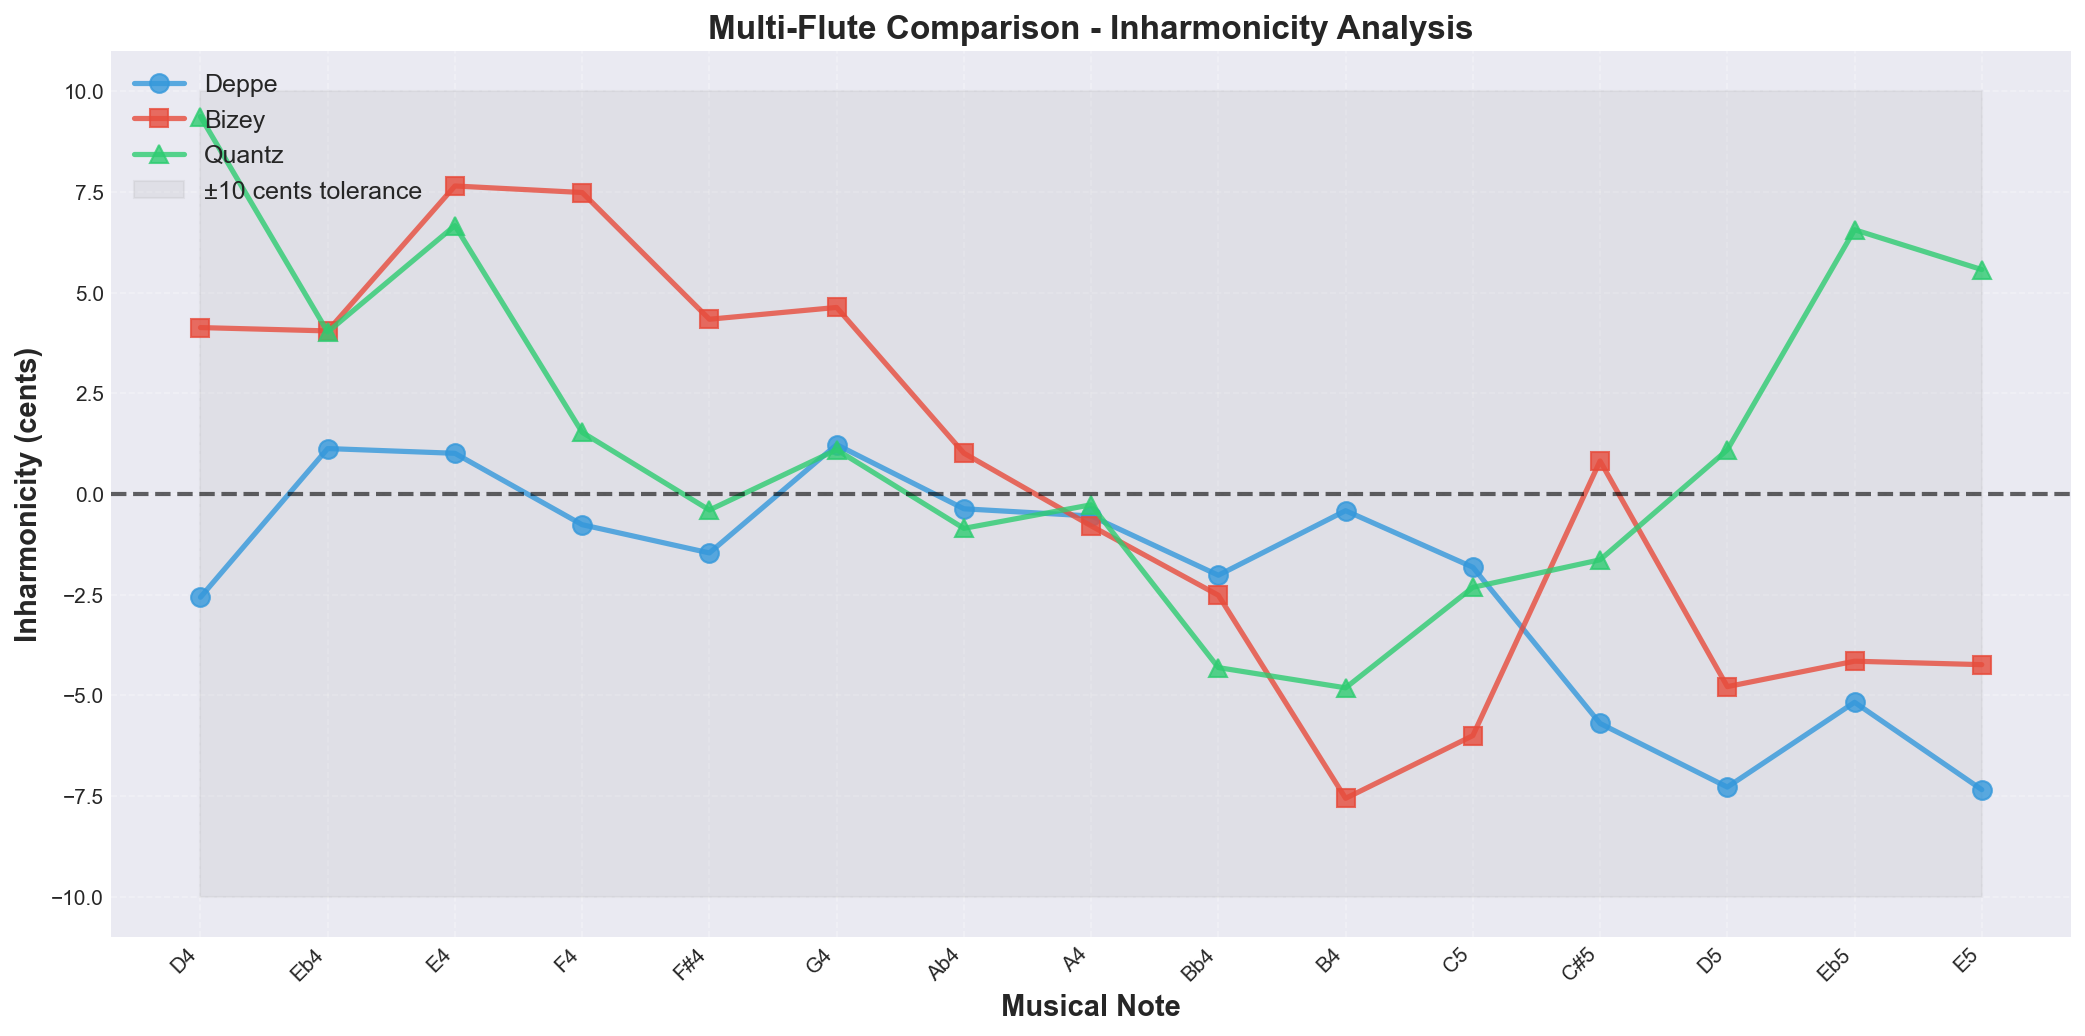
\includegraphics[width=0.7\textwidth]{presentation_screenshots/screenshot_multi_flute_comparison.png}
\end{figure}
\end{frame}

% ==================== SECTION 9: TECHNICAL DETAILS ====================
\section{Technical Implementation}

\begin{frame}{OpenWind Integration}
\textbf{Impedance Computation:}

\begin{itemize}
    \item \textbf{Geometry Preparation:}
    \begin{itemize}
        \item Bore segments: $[x_s, x_e, r_s, r_e, \text{type}]$
        \item Side holes with chimney heights
        \item Fingering charts
    \end{itemize}
    
    \item \textbf{Physical Parameters:}
    \begin{itemize}
        \item Speed of sound: $c(T) = 331.3\sqrt{1 + T/273.15}$
        \item Radiation impedance (unflanged/flanged)
        \item Wall losses (Webster-Lokshin model)
    \end{itemize}
    
    \item \textbf{Computation:}
    \begin{itemize}
        \item Transmission line method
        \item Frequency: 100-3000 Hz (configurable)
        \item Step: 2 Hz (default)
    \end{itemize}
\end{itemize}
\end{frame}

\begin{frame}{Data Flow}
\textbf{Processing Pipeline:}

\vspace{0.3cm}
\begin{enumerate}
    \item \textcolor{acousticblue}{\textbf{Input:}} JSON Files / Database
    \item \textcolor{acousticgreen}{\textbf{Processing:}}
    \begin{itemize}
        \item FluteData: Load and validate geometry
        \item OpenWind: Compute impedance
    \end{itemize}
    \item \textcolor{acousticorange}{\textbf{Analysis:}}
    \begin{itemize}
        \item FluteAnalyzer: Extract metrics
        \item Generate visualizations
        \item Generate reports
    \end{itemize}
\end{enumerate}

\vspace{0.3cm}
\begin{center}
\textit{All steps are cached in database for efficiency}
\end{center}

\textbf{Key Steps:}
\begin{enumerate}
    \item Load/validate geometry
    \item Prepare OpenWind inputs
    \item Compute impedance
    \item Extract metrics
    \item Generate visualizations
    \item Export reports
\end{enumerate}
\end{frame}

\begin{frame}{Performance Optimizations}
\textbf{Caching Strategy:}

\begin{itemize}
    \item \textbf{Database Caching:}
    \begin{itemize}
        \item Store impedance results with parameter hash
        \item Detect parameter changes
        \item Skip recalculation if parameters unchanged
    \end{itemize}
    
    \item \textbf{Lazy Loading:}
    \begin{itemize}
        \item 3D visualization loads only when accessed
        \item Large datasets loaded on demand
        \item Memory-efficient operation
    \end{itemize}
    
    \item \textbf{Parallel Processing:}
    \begin{itemize}
        \item Multi-flute analysis can be parallelized
        \item Sensitivity analysis variants computed independently
    \end{itemize}
\end{itemize}

\textbf{Typical Performance:}
\begin{itemize}
    \item Single flute analysis: 10-30 seconds
    \item Multi-flute comparison: Scales linearly
    \item Database retrieval: < 1 second (cached)
\end{itemize}
\end{frame}

% ==================== SECTION 10: APPLICATIONS ====================
\section{Applications \& Use Cases}

\begin{frame}{Research Applications}
\textbf{Academic Research:}

\begin{itemize}
    \item \textbf{Historical Instrument Analysis:}
    \begin{itemize}
        \item Compare instruments from different periods
        \item Study maker-specific characteristics
        \item Document acoustic evolution
    \end{itemize}
    
    \item \textbf{Design Studies:}
    \begin{itemize}
        \item Understand geometry-acoustics relationships
        \item Optimize for specific acoustic goals
        \item Validate theoretical models
    \end{itemize}
    
    \item \textbf{Player-Instrument Interaction:}
    \begin{itemize}
        \item Quantify compensation requirements
        \item Study register transition challenges
        \item Analyze playing difficulty metrics
    \end{itemize}
\end{itemize}
\end{frame}

\begin{frame}{Practical Applications}
\textbf{Instrument Making:}

\begin{itemize}
    \item \textbf{Design Optimization:}
    \begin{itemize}
        \item Sensitivity analysis guides design choices
        \item Identify critical vs. tolerant parameters
        \item Reduce trial-and-error iterations
    \end{itemize}
    
    \item \textbf{Quality Control:}
    \begin{itemize}
        \item Compare new instruments to references
        \item Identify manufacturing deviations
        \item Ensure consistency
    \end{itemize}
    
    \item \textbf{Reproduction:}
    \begin{itemize}
        \item Accurate geometric modeling
        \item Engineering drawings for manufacturing
        \item G-code for CNC machining
    \end{itemize}
\end{itemize}

\textbf{Education:}
\begin{itemize}
    \item Teaching acoustic principles
    \item Demonstrating geometric effects
    \item Interactive exploration tool
\end{itemize}
\end{frame}

% ==================== SECTION 11: FUTURE WORK ====================
\section{Future Directions}

\begin{frame}{Potential Enhancements}
\textbf{Planned Features:}

\begin{itemize}
    \item \textbf{Advanced Analysis:}
    \begin{itemize}
        \item Modal analysis (beyond impedance minima)
        \item Time-domain simulations
        \item Nonlinear effects modeling
    \end{itemize}
    
    \item \textbf{Machine Learning:}
    \begin{itemize}
        \item Predictive models for design optimization
        \item Pattern recognition in historical instruments
        \item Automated quality assessment
    \end{itemize}
    
    \item \textbf{Extended Instrument Support:}
    \begin{itemize}
        \item Other woodwind instruments
        \item Brass instruments
        \item Custom geometries
    \end{itemize}
    
    \item \textbf{Collaboration Features:}
    \begin{itemize}
        \item Cloud database sharing
        \item Collaborative analysis
        \item Version control integration
    \end{itemize}
\end{itemize}
\end{frame}

% ==================== CONCLUSION ====================
\section{Conclusion}

\begin{frame}{Summary}
\textbf{Key Strengths:}

\begin{enumerate}
    \item \textbf{Comprehensive Analysis:}
    \begin{itemize}
        \item Multiple acoustic metrics
        \item Novel resonator truncation method
        \item Sensitivity analysis capabilities
    \end{itemize}
    
    \item \textbf{User-Friendly Interface:}
    \begin{itemize}
        \item Intuitive PyQt5 GUI
        \item Interactive visualizations
        \item Detailed information buttons
    \end{itemize}
    
    \item \textbf{Scientific Rigor:}
    \begin{itemize}
        \item Based on established acoustic theory
        \item OpenWind integration
        \item Proper mathematical formulations
    \end{itemize}
    
    \item \textbf{Practical Tools:}
    \begin{itemize}
        \item Engineering drawings
        \item G-code generation
        \item Database management
    \end{itemize}
\end{enumerate}
\end{frame}

\begin{frame}{Thank You}
\begin{center}
\Large
\textbf{Questions \& Discussion}

\vspace{1cm}

\large
Software available for research collaboration

\vspace{0.5cm}

\normalsize
Contact: [Your contact information]
\end{center}
\end{frame}

\end{document}

